\documentclass{report}

\usepackage[margin=1in]{geometry}
\usepackage{amsmath,amsthm,amssymb}
\usepackage{enumitem}
\usepackage{graphicx}
\usepackage{caption}
\usepackage{mathtools}
\renewcommand{\familydefault}{\sfdefault}
\begin{document}
% ------------------------------------------ %
%                 START HERE                 %
% ------------------------------------------ %
\title{CS5785 Homework 1\\
\large{
    Applied Machine Learning
}
}


\author{
	Vijay Pillai\\
	Thomas Matecki}
\maketitle
\section*{Programming Exercises}

\begin{enumerate}
	\item Digit Recognizer
	\begin{enumerate}[label=(\alph*)]
		\item 
		Training and test data are located in files \textit{train.csv} and \textit{test.csv} respectively. The training data comprises 42000 images and the test data comprises 28000 images.

		\item Figure 1 is one of each digit(0-9) displayed as a 28 by 28 pixel grid.  
		\begin{center}
		\captionof{figure}{}
		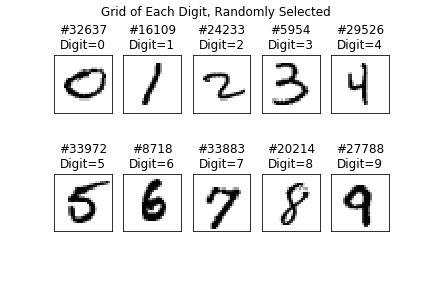
\includegraphics[width=12cm]{one_grid_x_each_digit.png}
		\end{center}
		\item The distribution of digits within the training data is nearly uniform.
		\begin{center}
		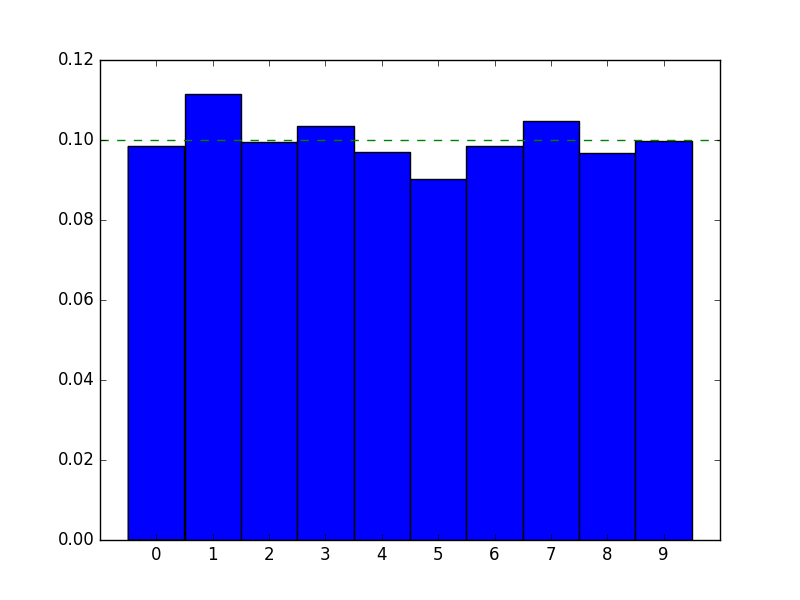
\includegraphics[width=12cm]{distrib.png}
		\end{center}
		
		\item 10 randomly picked digits and their closest matches are below.
		
		\begin{center}
		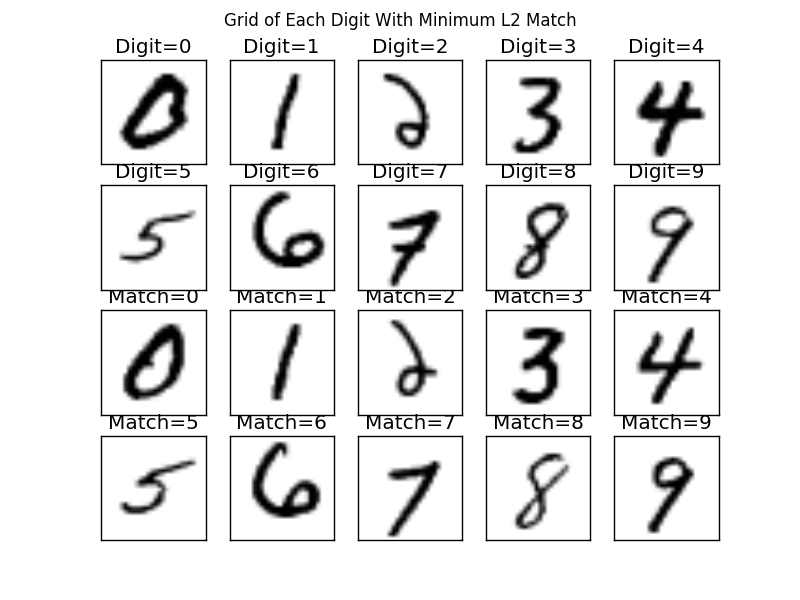
\includegraphics[width=12cm]{matches.png}
		\end{center}
		
		\item The confusion matrix for all digits is displayed below, with vertical axis is \textit{actual} and horizontal axis is \textit{predicted}.\\
		\begin{center}
		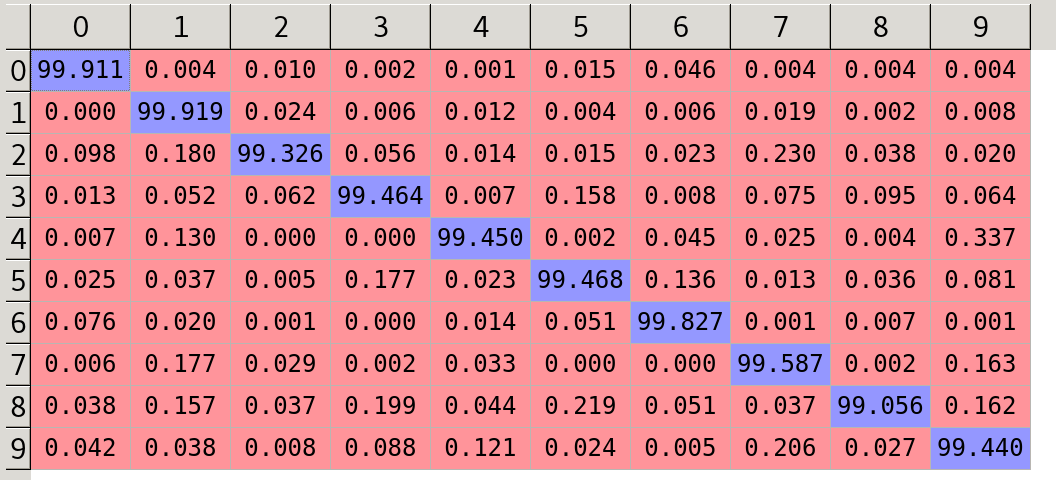
\includegraphics[width=12cm]{confusion_matrix.png}
		\end{center}
		
	\end{enumerate}
	\item The Titanic Disaster
	\begin{enumerate}[label=(\alph*)]
		\item The test datasets can be found in the \textit{./titanic\_data} directory.
		\item Implementation is completed using scipy's LogisticRegression class and can be found in file titanic.py. Two things to note about the implementation:
		\begin{itemize}
		\item The categoricaly features are translated to \textit{One Hot} encoding before the classifier is parsed.
		\item Features \textit{PassengerId, Name, Ticket Fare, Cabin}, and \textit{Embarked} are ommitted from the classifer.  Through some trial and error, one can draw the conclusion that omitting these features yields a more accurate classifier, most likely because they are scarcely populated(E.g. Cabin has values in the test set do not exist in the training data) or contain a a high number of unique, categorical values(E.g. Fare). The values thus increase the dimensionality of the model while offering nothing but idiosyncracies that likely exist only in the sample training data.
		\end{itemize}
		\item the result of the classifier have been submitted to kaggle and can be found in the \textit{./titanic\_data}. 
	\end{enumerate}
	
\end{enumerate}

\section*{Written Exercises}	
\begin{enumerate}
	\item Based on the defintions of variance and covariance,:\\
	\centerline{$var(X) = E[(X - E[X])^2]$}
	\centerline{$cov(X) = E[(Y - E[Y])(X - E[X])$}
	we have:
	\begin{align*}
    var[X-Y] &= E[( X - Y - E[X - Y])^2]  \\
    	 	 &= E[( X - Y - E[X] - E[Y])^2] \\
    	 	 &= E[( X - E[X]) - (Y - E[Y]) )^2] \\
    	 	 &= E[( X - E[X])^2 - 2E[(Y - E[Y])(X - E[X])] + E[(Y - E[Y])^2]] \\
    	 	 &= var(X) + var(Y) - 2E[(Y - E[Y])(X - E[X])] \\
    	 	 &= var(X) + var(Y) - 2cov(X,Y ) \\
    \end{align*}
	\item Letting event R be a positive test result, and event D be the occurence of a defective widget, we have...
	\begin{align*}
	     & P(D) = \frac{1}{100,000} \\
	     & P(R \vert D) = .95  \\
	     & P(\lnot R \vert \lnot D) = .95 \\
	 \end{align*}
	    ...and therefore...
	    \begin{align*}
	     & P(\lnot D) 				= 1 - \frac{1}{100,000} = \frac{99,999}{100,000} \\
	     & P(\lnot R \vert 		D) 	= 1-  P(R \vert D) =.05  & 
	     \text{(because $R \cap \lnot R = \emptyset$)}\\
	     & P(R 		\vert \lnot D) 	= .05  \\
	 	\end{align*}
	 	Additionally, the probability of a positive test result is the sum of the probabilities of a  defective widget testing positive and a non-defective widget testing positive; i.e.,
	 	\begin{align*}
	 	 P(R) 	&= P(R \cap D) + P(R \cap \lnot D)\\
	 	 		&= P(R \vert D)P(D) + P(R \vert \lnot D)P(\lnot D) \\
	 	 		&= (.95)\frac{1}{100,000} + (.05)\frac{99,999}{100,000} 
	 	 		 = \frac{.95}{100,000} + \frac{4999.95}{100,000} 
	 	 		 = \mathbf{\frac{5000.9}{100,000}}\\
	    \end{align*}
	    
	     
	    \begin{enumerate}[label=(\alph*)]
		\item Given a positive test result, the probability the widget is actually defective is:
	 	\begin{align*}
	 	 P(D \vert R)	&= \frac{P(R \vert D)P(D)}{P(R)} & \text{(bayes rule)} \\
	 	 				&= \frac{\frac{.95}{100,000}}{\frac{5000.9}{100,000}}
	 	 				 = \mathbf{0.000189966}
	    \end{align*}
		\item The probability a widget is not defective and tests positive is:
		\begin{align*}
		P(R \cap \lnot D) = P(R \vert \lnot D)P(\lnot D) 	&= (.05)\frac{99,999}{100,000} \\
															&= 0.0499995
		\end{align*}
		The probability a widget is defective and does not test positive is:
		\begin{align*}
		P(\lnot R \cap D) = P(\lnot R \vert  D)P(D) 	&= \frac{.05}{100,000} \\
														&= 0.0000005
		\end{align*}
		Therefore 499995 non-defective widgets are thrown out and 5 defective widgets are shipped per year.
		\end{enumerate}
		\item For KNN classification with $n$ data points...
		\begin{enumerate}
			\item When $k = n$, all data points are considered for any prediction, and therefore any prediction will simply yield the prior probability of the training data. As k approaches 1, fewer training points are taken in to consideration for a prediction, therfore, as $k \rightarrow n$ the mean squared predicion error decreases.
			\item  Removing half of the training data lowers the \textit{density} of the training sample. This means that for any test point $x$, it's \textit{nearest neighbors}($x_i \in N_k$) will be, on average, farther away(or less similiar to $x$). To maintain a consistent \textit{variance}, the value of $k$ must be descreased by a factor of $2$. 
			
			\item If we have a data set containing $n$ datapoints, the relative computational cost $C_i$, of performing cross validation, as a function of $i$ folds can be expressed as:
			
			\begin{equation*}
			 C = i \left( \frac{n}{i} \right)\left( \frac{n(i-1}{i} \right) =  \frac{n^2(i-1)}{i}
			\end{equation*}
			
			Extending our conclusion from (b), candidates for $k$ should be tested with an adjustment proportional to $\frac{i-1}{i}$ (specifically - adjust k according to the change in density that occurs when removing $\frac{1}{i}$th of the samples form the training data - see (e) one may also consider the dimensionality, of the feature vector, $x$). \\
			
			Choosing $i$ to be large (say 10), will mitigate the impact of density reduction, however the larger $i$ is more computationally expensive($i \rightarrow \infty, C_i \rightarrow n^2$).
						
			\item If $k$ is large, for some $x$ it may be beneficial to weigh votes from a neighbor $N_k(x)$ using some function $w$ that decreases as the distance $d$, from $x$ increases. E.g.:
			\begin{equation*}
				w_{k}(x,N_k(x) = \frac{1}{1 + d(x,N_k(x) )}
			\end{equation*}
			
			\item As the dimension of a model increases, the \textit{closeness} of a point of it's neighbors decreases. That is the the size of neighborhood about a point does not scale linearly with the fraction of each each input dimension needed to cover that neighbor hood. If we consider the unit space in 1, 2, and 3 dimensions and create a subspace that is half of the input the unit spaces for each dimension, then the respective volume is $\frac{1}{2}$, $\frac{1}{4}$, and $\frac{1}{8}$. The inverse is also true; to maintain a fixed fraction of the total space, a large interval of each dimension must be considered. Additionally, the stability of the KNN algorithm relies upon a dense training sample. For a fixed number of points in dimension $N$, increasing the dimension by $p'$ requires a an increase in the number of data points on the order of to $N^\frac{1}{p'}$
		\end{enumerate}
		
	
\end{enumerate}

\end{document}
 